\section{Referencial Teórico}
	\label{sec:referencial}
	
%%%%%%%%%%
% Retomada das Definições
%%%%%%%%%%	
%
% Documento é uma sucessão de assuntos
%%% 
Um documento textual, sobre tudo quando longo, é frequentemente uma sucessão de assuntos. 
%
% Segmentação
%%% 
A segmentação textual ou segmentação topical é a tarefa de dividir um texto mantendo em cada parte um tópico com seu significado completo.
	


%%%%%%%%%%%%%%%
% Unidades de Informação 
%%%%%%%%%%%%%%% 
%
% O texto deve ser divido em unidades que não pode ser dividida entre segmentos 
%%% 
O texto deve ser previamente dividido em unidades de informação, que podem ser palavras, paragrafos e mais usualmente em sentenças. Essas unidades são processadas pelos algoritmos como a menor parte de um segmento, ou seja uma unidade não pode divida, mas deve pertencer integralmente a um segmento.
%
% Exemplos 
%%% 
Por exemplo, algoritmos baseados em janelas deslizantes, avançam uma unidade a cada passo. Da mesma forma, algoritmos baseados em matrizes de similaridade, devem calcular a similaridade entre essas unidades.

%
% Sentaças são mais usuais 
%%% 
Usualmente, utiliza-se sentenças como unidades informação, ou seja, as janelas deslizam uma sentença a cada passo e matrizes de similaridades armazenam as similaridades entre as sentenças do texto.
%
% O ponto entre unidades é um limite 
%%% 
Assim, cada ponto entre duas sentenças e considerado um candidato a limite entre segmentos.
  
%%%%%%%%%%
% Segmento
%%%%%%%%%%	
Dessa forma, um segmento pode ser visto como uma sucessão de unidades de informação que compartilham o mesmo assunto. 



%%%%%%%%%%
% Coesão léxica como **presuposto básico**
%%%%%%%%%%
Trabalhos anteriores se apoiam na ideia de que a mudança de tópicos em um texto é acompanhada de uma proporcional mudança de vocabulário, essa ideia, chamada de coesão léxica, sugere que a distribuição das palavras é um forte indicador da estrutura do texto. A partir disso, vários algoritmos foram propostos baseados na ideia de que um segmento pode ser identificado e delimitado pela análise das palavras que o compõe~\cite{Galley2003}~\cite{Boguraev2000}.



%, bem como é necessário mensurar suas similaridades. { asunidades de medida}

%%%%%%%%%%
% Porque cosseno
%%%%%%%%%%
Uma vez que a coesão léxica é pressuposto básico da maioria dos algoritmos, o cálculo da similaridade entre unidades de informação (comumente sentenças) é fundamental. Uma medida de similidade frequentemente utilizada é o cosseno, apresentada na Equação~\ref{equ:cosine}, onde $f_{x,j}$ a frequência da palavra $j$ na sentença $x$ e $f_{y,j}$ sendo a frequência da palavra $j$ na sentença $y$.


\begin{equation}
Sim(x,y) = \frac
{\Sigma_j f_{x,j} \times f_{y,j}}
{\sqrt{\Sigma_j f^2_{x,j} \times \Sigma f^2_{y,j}}}
\label{equ:cosine}
\end{equation}


\subsection{Principais algoritmos}
	\label{subsec:principaisalgoritimos}

Entre os principais trabalhos da literatura podemos citar o  \textit{TextTiling}~\cite{Hearst1994} e o \textit{C99}~\cite{Choi2000}.
%
%%%%%%%%%%%%%%%%%%%%%%%%%%%%%%%%%%%%%%%%%%%%%%%
%%%              TextTiling                 %%%
%%%%%%%%%%%%%%%%%%%%%%%%%%%%%%%%%%%%%%%%%%%%%%%
O \textit{TextTiling} é um algoritmo baseado em janelas deslizantes, onde para cada candidato a limite, analisa-se o texto circundante. Um limite ou quebra de segmento é identificado quando sempre que a similaridade cai abaixo de um limiar.
% \textit{threshold}. %TODO - explicar como se encontra os vales


O \textit{TextTiling} recebe uma lista de candidatos a limite, usualmente finais de parágrafo ou finais de sentenças. Para cada posição candidata são construídos 2 blocos, um contendo sentenças que a precedem e outro com as que a sucedem. O tamanho desses blocos é um parâmetro a ser fornecido ao algoritmo e determina o tamanho mínimo de um segmento.
%
Em seguida, os blocos de texto são representados por vetores que contém as frequências de suas palavras. Então, usa-se cosseno (Equação~\ref{equ:cosine}) para calcular a similaridade entre os blocos adjacentes a cada candidato e identifica-se uma transição entre tópicos pelos vales na curva de dissimilaridade.

%TODO como apresentado na Figura~\ref{fig:curvadedissimilaridade}.


O \textit{TextTiling} possui menor complexidade computacional. Por outro lado, algoritmos mais complexos apresentam acurácia relativamente superior como apresentado em~\cite{Choi2000, Kern2009, Misra2009}.




%%%%%%%%%%%%%%%%%%%%%%%%%%%%%%%%%%%%%%%%%%%%%%%
%%%                  C99                    %%%
%%%%%%%%%%%%%%%%%%%%%%%%%%%%%%%%%%%%%%%%%%%%%%%

Choi \cite{Choi2000} apresenta um algoritmo baseado em ranking, o \textit{C99}. 
%
Embora muitos trabalhos utilizem matrizes de similaridades, o autor traz obervações.
%
Ele aponta que para pequenos segmentos, o cálculo de suas similaridades não é confiável, pois uma ocorrência adicional de uma palavra causa um impacto que pode alterar significativamente o cálculo da similaridade.
%
Além disso, o estilo da escrita pode não ser constante em todo o texto. Choi sugere que, por exemplo, textos iniciais dedicados a introdução costumam apresentar menor coesão do que trechos dedicados a um tópico específico. Portanto, comparar a similaridade entre trechos de diferentes regiões não é apropriado.
% Complexidade O(n²)
Devido a isso, as similaridades não podem ser comparadas em valores absolutos. Então, o autor contorna esse problema fazendo uso de \textit{rankings} de similaridade para encontrar os segmentos de texto. 


Inicialmente é construída uma matriz que contém as similaridades de todas as unidades de texto. Em seguida, cada valor na matriz de similaridade é substituído por seu ranking local. Onde para cada elemento da matiz, seu \textit{ranking} é o número de elementos vizinhos com valor de similaridade menor que o seu.

% O que é a máscara
Então, para cada elemento delimita-se uma região da matriz, denominada máscara, para comparar com seus vizinhos.
%
Na Figura~\ref{fig:exemplomatrixrank} é apresentado um quadro de dimensões 3~x~3 destacado na matriz de similaridades, que contém os valores $\{0,3; 0,4; 0,4; 0,6; 0,5; 0,2; 0,9; 0,5; 0,7\}$, onde cada elemento da matrix é a similaridade entre duas unidades de informação. Tomando como exemplo o elemento com valor $0,5$, a mesma posição na matriz de \textit{ranks} terá o valor $4$, pois esse é o número de vizinhos com valores inferiores a $0,5$ dentro do quadro analisado na matriz de similaridades. 


  \begin{figure}[!h]

	\centering
	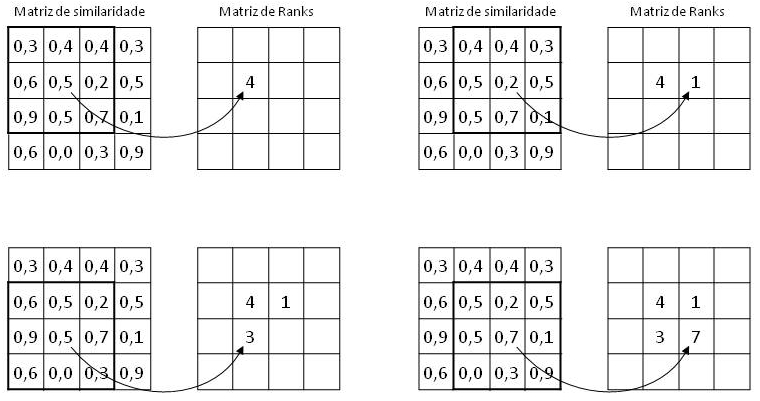
\includegraphics[width=0.45\textwidth]{exemplo-matrix-rank-noborder.jpg}
	\caption{Exemplo de construção de uma matriz de rank.~\cite{Choi2000}}
	\label{fig:exemplomatrixrank}

  \end{figure}



Finalmente, utiliza um método de divisão por \textit{clustering} baseado no algoritmo de maximização de Reynar~\cite{Reynar1998} para identificar os limites entre os segmentos. 




\subsection{Segmentação de Referência} % Recordado da seção Documentos em 15-06-2017


%%%%%%%%%% 
% Necessidade de uma referência
%%%%%%%%%%
Para que se possa avaliar um segmentador automático de textos é preciso uma referência, isto é, um texto com os limites entre os segmento conhecidos. Essa referência, deve ser confiável, sendo uma segmentação legítima que é capaz de dividir o texto em porções relativamente independentes, ou seja, uma segmentação ideal.



%%%%%%%%%%
% Formas de conseguir a Segentanção de Referência
%%%%%%%%%%
Entre as abordagens mais comuns para se conseguir essas referências, encontramos: 

\begin{itemize}

% Concatenação
\item A concatenação aleatória de documentos distintos, onde o ponto entre o final de um texto e o início do seguinte é um limite entre eles. 

% Segmentação manual
\item A segmentação manual dos documentos, nesse caso, pessoas capacitadas, também chamadas de juízes, ou mesmo o autor do texto, são consultadas e indicam manualmente onde há uma quebra de segmento. 
% Mediador em conversas
\item Em transcrição de conversas faladas em reuniões com múltiplos participantes, um mediador é responsável por encerrar um assunto e iniciar um novo, nesse caso o mediador anota manualmente o tempo onde há uma transição de tópico. 

\end{itemize}

% Não avaliar
Em aplicações onde a segmentação é uma tarefa secundária e quando essas abordagens são custosas ou não se aplicam, é possível, ao invés de avaliar o segmentador, analisar seu impacto na aplicação final.










\subsection{Medidas de Avaliação}

%%%%%%%%%%%%%%%
% Medidas de avaliação tradicionais 
%%%%%%%%%%%%%%%
%
% Utilizadas em RI e Classificação 
%%% 
As medidas de avaliação tradicionais como precisão e revocação são usadas em recuperação de informação e classificação automática para medir o desempenho de modelos de classificação e predição. São baseadas na comparação dos valores produzidos por uma hipótese com os valores reais. 


%
% Baseadas em Matriz de Confusão 
%%% 
Esses valores são apresentados em uma tabela que permite a visualização do desempenho de um algoritmo, a qual é chamada de matriz de confusão. Na Tabela~\ref{tab:matrizconfusao} é apresentada a matriz de confusão para duas classes (Positivo e Negativo).

%Uma matriz de confusão é uma tabela que permite a visualização do desempenho de um algoritmo. 

\begin{table}[!h]
	\centering
	
	\begin{tabular}{|c|c|c|}
		\hline
		                & Predição Positiva         & Predição Negativa        \\ \hline
		Positivo real   & VP (Verdadeiro Positivo)  & FN (Falso Negativo)      \\ \hline
		Negativo real   & FP (Falso Positivo)       & VN (Verdadeiro Negativo) \\ \hline
	
	\end{tabular}
	
	\caption{Matriz de confusão.}
	\label{tab:matrizconfusao}

\end{table}


%%%%%%%%%%
%	Avaliações baseadas em hits 
%%%%%%%%%%
Essas medidas de avaliação tentam computar os erros do algoritmo, isto é, falsos positivos e falsos negativos, a fim de calcular seu desempenho. 

%
% Falso Positivo 
%%%
No contexto de segmentação textual, um falso positivo é um limite identificado pelo algoritmo que não corresponde a nenhum limite na segmentação de referência, ou seja, o algoritmo indicou que em determinado ponto há uma quebra de segmento, mas na segmentação de referência, no mesmo ponto, não há. 

%
% Falso Negativo 
%%% 
De maneira semelhante, um falso negativo é quando o algoritmo não identifica um limite existente na segmentação de referência, ou seja, em determinado ponto há, na segmentação de referência, um limite entre segmentos, contudo, o algoritmo não o identificou.

%
% Verdadeiro Positivo 
%%% 
Um verdadeiro positivo é um ponto no texto indicado pelo algoritmo e pela segmentação de referência como uma quebra de segmentos, ou seja, o algoritmo e a referência concordam que em determinado ponto há uma transição de assunto.

%
% O Verdadeiro Negativo, que não existe 
%%%
Na avaliação de segmentadores, não há o conceito de verdadeiro negativo. Este seria um ponto no texto indicado pelo algoritmo e pela segmentação de referência onde não há uma quebra de segmentos. Uma vez que os algoritmos apenas indicam onde há um limite, essa medida não é necessária. % Não há ou não e necessário?



Nesse sentido, 
%%%%%%%%%%%%%%%
% Precisão 
%%%%%%%%%%%%%%%
%
% Definição 
%%% 
a precisão, é a proporção de limites corretamente identificados pelo algoritmo. 
%
% Cálculo 
%%% 
É calculada dividindo-se o número de limites identificados automaticamente pelo número de candidatos a limite(Equação~\ref{equ:precisao}).
% 
\begin{equation}
	Presis\tilde{a}o = \frac{VP}{VP+FP}
	\label{equ:precisao}
\end{equation}
%
% Ideia 
%%% 
Essa medida varia entre $0,0$ e $1,0$, que indica a proporção de limites identificados pelo algoritmo que são corretos, ou seja, correspondem a um limite real na segmentação de referência. Porém não diz nada sobre quantos limites reais existem. 



%%%%%%%%%%%%%%%
% Revocação 
%%%%%%%%%%%%%%% 
%
% Definição 
%%% 
A revocação, é a proporção de limites verdadeiros que foram identificados pelo algoritmo.
%
% Cálculo 
%%%
É calculada dividindo-se o número de limites identificados automaticamente pelo número limites verdadeiros.


% 
\begin{equation}
	Revo\c{c}\tilde{a}o = \frac{VP}{VP+FN}
	\label{equ:revocacao}
\end{equation}
%
% Ideia 
%%% 
Pode variar entre $0,0$ e $1,0$, onde indica que a proporção de limites corretos que foram identificados. Porém não diz nada sobre quantos limites foram indentificados incorretamente. 

%%%%%%%%%%%%%%%
% Relação inversa entre precisão e revocação 
%%%%%%%%%%%%%%% 
Existe uma relação inversa entre precisão e revocação. Conforme o algoritmo aponta mais segmentos no texto, este tende a melhorar a revocação e ao mesmo tempo, reduzir a precisão. 
%
% Pode ser contornado com F1 
%%% 
Esse problema de avaliação pode ser contornado utilizado a medida $F^1$ que é a média harmônica entre precisão e revocação onde ambas tem o mesmo peso. 

%%%%%%%%%%%%%%%
% Medidas que consideram a distancia entre os segmentos 
%%%%%%%%%%%%%%% 
Além dessas medidas, que consideram apenas se um segmento foi corretamente definido, pode-se também considerar a distância entre o segmento extraído automaticamente e o segmento de referência~\cite{Kern2009}.


Na Figura~\ref{fig:exemplosegmentacaozoom} é apresentado um exemplo com duas segmentações extraídas automaticamente e uma referência. Em ambos os casos não há nenhum verdadeiro positivo, o que implica em zero para os valores de precisão, acurácia, e revocação, embora a segunda hipótese possa ser considerada superior à primeira se levado em conta a proximidade dos limites.



  \begin{figure}[!h]

	\centering
	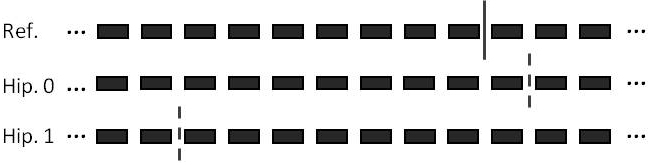
\includegraphics[width=0.47\textwidth]{windiffzoom.jpg}
	\caption{Exemplos de \textit{near missing} e falso positivo puro. Os blocos indicam uma unidade de informação e as linha verticais representam os limites entre segmentos de texto representando um tópico do texto. }
	\label{fig:exemplosegmentacaozoom}

  \end{figure}
  

Considerando o conceito de \textit{near misses}, algumas soluções foram propostas. As medidas de avaliação mais utilizadas são:

\begin{enumerate}

%%%%%%%%%%%%%%%
% Pk 
%%%%%%%%%%%%%%% 
%\item Em~\cite{Beeferman1999} é apresentada uma medida denominada P$_k$, 
%

\item P$_k$, proposta por Beeferman~\cite{Beeferman1999}, 
% Valores Parciais 
%%% 
atribui valores parciais a \textit{near misses}, ou seja, limites sempre receberão um peso proporcional à sua proximidade, desde que dentro de um janela de tamanho~$k$.
%
% Funcionamento 
%%% 
Para isso, esse método move uma janela de tamanho $k$ ao longo do texto. 
%
% Compara hipotese e referência		
%%% 
A cada passo verifica, na referência e na hipótese, se o início e o final da janela estão ou não dentro do mesmo segmento,
%
% Penalisa em caso de discrepânica 
%%% 
então, penaliza o algoritmo caso não concorde com a referência. Ou seja, dado duas palavras de distancia $k$, o algoritmo é penalizado quando não concordar com a segmentação de referência se as palavras estão ou não no mesmo segmento.
%
% Calculo de k 
%%% 
O valor de $k$ é calculado como a metade da média dos comprimentos dos segmentos reais. Como resultado, é retornado a contagem de discrepâncias divida pelo quantidade de segmentações analisadas. 
%
% Medida de dissimilaridade e interpretação 
%%% 
P$_k$ é uma medida de dissimilaridade entre as segmentações e pode ser interpretada como a probabilidade de duas sentenças extraídas aleatoriamente pertencerem ao mesmo segmento.

%%%%%%%%%%%%%%%
% WindowDiff 
%%%%%%%%%%%%%%% 
\item \textit{WindowDiff}. Pevzner~\cite{Pevzner2002} 
%
% Medida alternativa que considera outros aspectos 
%%%
apresenta uma medida alternativa à P$_k$~\cite{Beeferman1999} a fim de melhorar alguns aspectos. 
%
% Funcionamento do Windiff 
%%% 
De maneira semelhante, move uam janela pelo texto e penaliza o algoritmo sempre que o número de limites proposto pelo algoritmo não conicidir com o número de limites epeperados para aquela janela. Ou seja, o algoritmo é penalizado quando não concordar com a segmentação de referência quanto ao número de segmentos na janela. 
%
% Solução para considerar o tamanho das sentenças 
%%% 
Assim, consegue manter a sensiblidade a \textit{near misses} e além disso, considerar o tamanho das janelas.
%
% Solução para equilibrar falsos positivos e near missses 
%%% 
A fim de melhor equilibrar o peso dos falsos positivos em relação a \textit{near misses}, dobra-se a penalidade para falsos positivos, evitando-se a suparvalorização dessa medida. 
% OBS: Os problemas de Pk ficaram subentendidos aqui :/ 


\end{enumerate}







%
% Problemas do Pk 
%%% 
% aponta problemas na avaliação mais tradicional, P$_k$~\cite{Beeferman1999}. Eles apontam que esse método penaliza demasiadamente os falsos negativos em relação aos falsos positivos e a \textit{near misses}, além disso, desconsidera o tamanho dos segmentos. 
%
% Soluções do WinDiff 
%%%
% Como solução, propõem um método, que traz duas diferenças principais: a dobra da penalidade para os falsos positivos a fim de diminuir o problema da subestimação dessa medida e, diferente de P$_k$, ao mover a janela pelo texto, penaliza-se o algoritmo sempre que o número de limites proposto pelo algoritmo não coincidir com o número de limites esperados para aquela janela de texto. 

% Com isso, demonstram em seu trabalho que, em relação a P$_k$, \textit{WindowDiff} consegue resolver seus principais problemas e mantém sua proposta inicial de sensibilidade a \textit{near misses}, penalizando-os menos que os falsos positivos puros.




%nesse exemplo, o valor $0,5$ é substituído por $4$ na matriz de ranks pois há 4 vizinhos com valor inferior
%, o qual é calculado com a Equação~\ref{equ:ranklocal}. 

%o valor $0,5$ é comparado com seus elementos vizinhos, o


%Um exemplo é mostrado na Figura \ref{fig:exemplomatrixrank} abaixo, onde utiliza-se uma máscara de largura igual a 3.



%Por por outro lado, tem a desvantagem de ser mais difícil de interpretar. 
%As medidas apresentadas acima falham ao não serem sensíveis a \textit{near misses}, ou seja, quando um limite não coincide exatamente com o esperado, mas está próximo a ele~\cite{Kern2009}. --> Reescrito por Rafael.



%

% 1 cria uma matrix de similaridades
% 2 cria a matrix de ranking
% 3 aplica divisive clustering

% mask = quadro
% pegar um exemplo --> mostrar os numeros dentro do quatro e pq o resultado foi aquele

% colocar os passos na imagem


%Ela propõe um algoritmo baseado em janelas deslizante, para analisar blocos de texto adjacentes e identificar os limites com base nas similaridades dos blocos.

% baixa complexidade computacional devido a simplicidade do algoritmo e baixa eficiência quando comparado a outros métodos mais sofisticados como apresentados em~\cite{Choi2000, Kern2009, Misra2009}.



% portanto são consideradas candidatas a limite entre segmentos.

% Uma unidade pode ser, por exemplo, palavras, sentenças ou parágrafos devem compartilhar o mesmo assunto.
% que compartilham um assunto. 


%apontam que a coesão léxica é um forte indicador da estrutura do texto, isto é, a mudança de tópicos é acompanhada de uma proporcional mudança de vocabulário. A partir disso, vários algoritmos foram propostos baseados na ideia de que um segmento pode ser identificado e delimitado pela análise das palavras que o compõe~\cite{Galley2003}~\cite{Boguraev2000}.


%\begin{equation}
%r(x,y) = \frac
%{Numero\ de\ elementos\ com\ similaridade\ menor}
%{Numero\ de\ elementos\ examinados}
%\label{equ:ranklocal}
%\end{equation}


% Clustering Reynar maximization
	

%Finalmente, os limites são identificados sempre que a similaridade entre blocos adjacentes entre cada candidato ultrapassa um determinado \textit{threshold}.



% Mensionar que existem duas abordagens principais - Baseada em coesão léxiam e em discursos [ver a pg 2 do Text Segmentation With Topic Moeling and Entity Coherence]

%Essa abordagem apresenta uma redução taxa de erros de 22\% para 10\%. Por outro lado, exige que a quantidade de segmentos seja conhecida.
%Como melhoramento, os autores apresentam posteriormente uma versão do \textit{C99} que utiliza \textit{Latent Semantic Analisys} (LSA) para calcular as similaridades ao invês de cosseno~\cite{Choi2001-LSA}.







%Há ainda outros critérios para segmentação como a segmentação temática 

%outros tipos de abordagem
%	Segmentação funcional
%	Segementação temática


% número de predições corretas com número de total predições

% apresenta um esquema de \textit{rankings} para contornar esse problema.


% As medidas de avaliação tradicionais baseiam se na contagem de acertos. Quando um fim de segmento extraído automaticamente coincide com o limite de referência, têm-se um acerto.

% Essa medida varia entre $0,0$ e $1,0$, sendo $1,0$ uma pontuação onde todos os limites identificados pelo algoritmo são corretos, ou seja, correspondem a um limite real na segmentação de referência. Porém não diz nada sobre quantos limites reais existem. 


% As medidas de avaliação tradicionais baseiam se na contagem de acertos. Quando um fim de segmento extraído automaticamente coincide com o limite de referência, têm-se um acerto.
% https://mineracaodedados.wordpress.com/tag/matriz-de-confusao/


% 		este e a referência não concordam se as palavras estão ou não no mesmo segmento.  uma discrepância é computada quando o algoritmo e a referência não concordam se as palavras estão ou não no mesmo segmento.


% \item \textit{WindowDiff}. Pevzner~\cite{Pevzner2002} aponta problemas na avaliação mais tradicional, P$_k$~\cite{Beeferman1999}. Eles apontam que esse método penaliza demasiadamente os falsos negativos em relação aos falsos positivos e a \textit{near misses}, além disso, desconsidera o tamanho dos segmentos. Como solução, propõem um método, que traz duas diferenças principais: a dobra da penalidade para os falsos positivos a fim de diminuir o problema da subestimação dessa medida e, diferente de P$_k$, ao mover a janela pelo texto, penaliza-se o algoritmo sempre que o número de limites proposto pelo algoritmo não coincidir com o número de limites esperados para aquela janela de texto. 

%  \begin{figure}[!h]
%
%	\centering
%	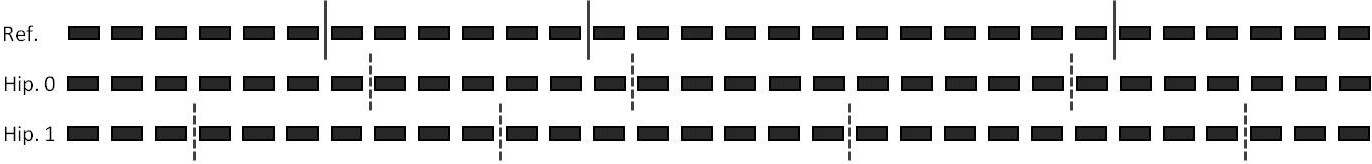
\includegraphics[width=0.47\textwidth]{windiff.jpg}
%	\caption{
%	Exemplo de duas segmentações hipotéticas em comparação a uma ideal. 
%	}
%	\label{fig:exemplosegmentacao}
%
%  \end{figure}
  

